\documentclass[border=10pt]{standalone}

\usepackage{tikz}
\usepackage{tikzsymbols}
\usetikzlibrary{calc,patterns,shapes.geometric}

\def\centerarc[#1](#2)(#3:#4:#5){\draw[#1] ($(#2)+({#5*cos(#3)},{#5*sin(#3)})$) arc (#3:#4:#5);}

\begin{document}
	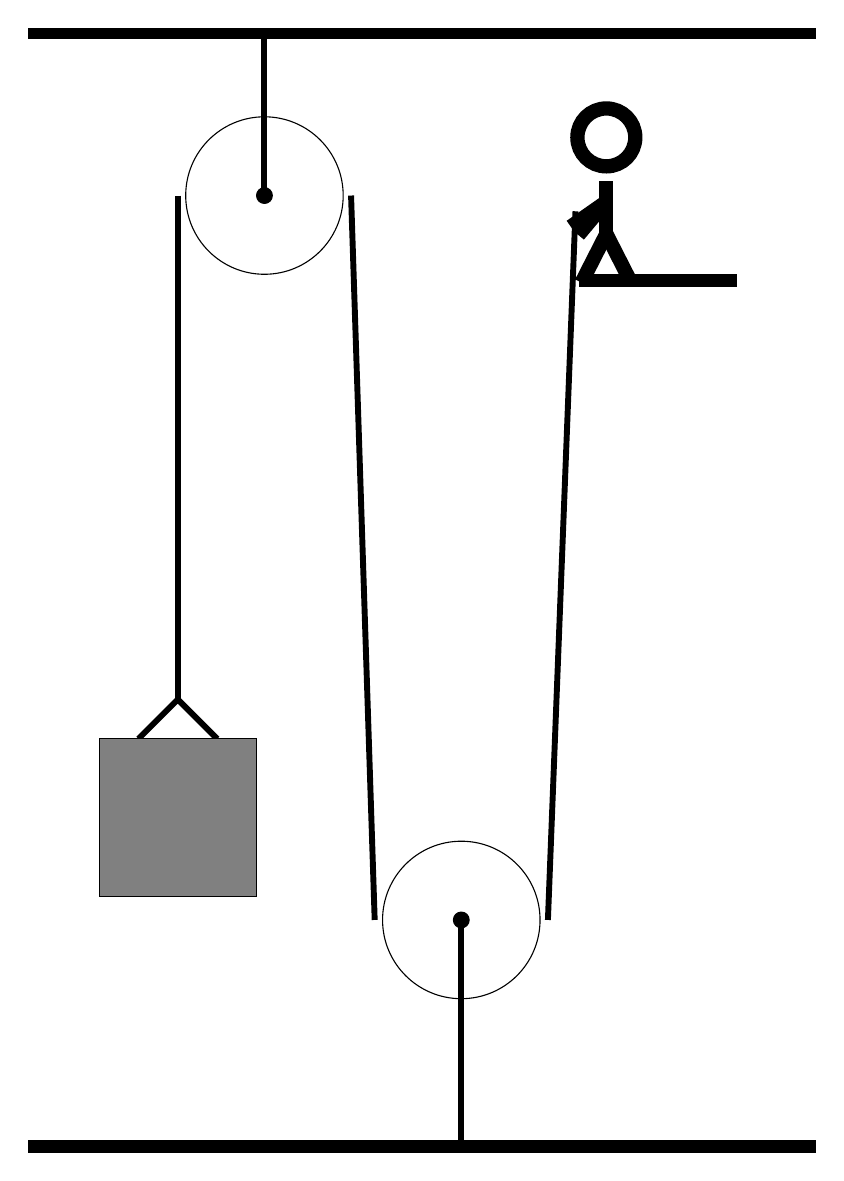
\begin{tikzpicture}
		%%%%% START %%%%%
		\draw[fill=black] (-2, 14) rectangle (8, 14.125);
		
		\draw (3.5, 2.8) circle (1);
		\draw[fill=black] (3.5, 2.8) circle (0.1);
		\draw[line width=0.75mm] (3.5, 2.8) -- (3.5, 0);
		
		\draw (1, 12) circle (1);
		\draw[fill=black] (1, 12) circle (0.1);
		\draw[line width=0.75mm] (1, 14) -- (1, 12);
		
		\draw[line width=0.75mm](-0.6, 5.1) --  (-0.1, 5.6) -- (0.4, 5.1);
		\draw[fill=black!50] (-1.1, 5.1) rectangle (0.9, 3.1);
		
		\draw[line width=0.75mm](-0.1, 12) -- (-0.1, 5.6);
		\centerarc[line width=0.75mm](1, 12)(180:0:1.1)
		\draw[line width=0.75mm](2.1, 12) -- (2.4, 2.8);
		\centerarc[line width=0.75mm](3.5, 2.8)(180:360:1.1)
		\draw[line width=0.75mm](4.6, 2.8) -- (4.95, 11.8);
		
		\node at (5.3, 12) {\Strichmaxerl[10][35][-130]};
		\draw[fill=black] (5, 11) rectangle (7, 10.85);
		
		\draw[fill=black] (-2, 0) rectangle (8, -0.15);
		%%%%% END %%%%%
	\end{tikzpicture}
\end{document}